\chapter{Tập hợp số tự nhiên}

\section{Tập hợp số tự nhiên}

\subsection{KIẾN THỨC CẦN NHỚ}
\subsubsection{Tập hợp}
\immini{\textit{Khái niệm tập hợp:} Một \textbf{tập hợp} (gọi tắt là tập) bao gồm những đối tượng nhất định. Các đối tượng đó được gọi là \textbf{phần tử} của tập hợp. 

Hình vẽ bên: $A$ là tên tập hợp, $x$ là một phần tử của tập $A$ (ta còn nói $x$ nằm trong $A$ hoặc $A$ chứa $x$), kí hiệu $x\in A$; $y$ không thuộc tập $A$, kí hiệu $y\notin A$.}{
	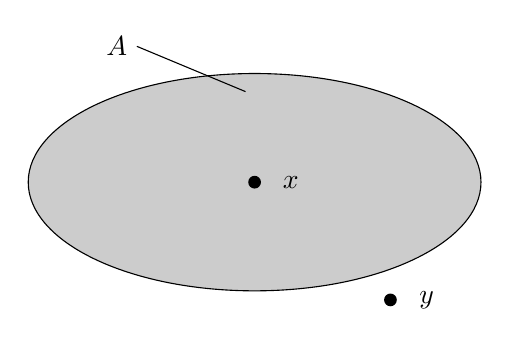
\begin{tikzpicture}[scale=1.15]
		\draw[fill=gray!40]
		(0:0) ellipse ({2.5} and {1.2})
		;
		\draw
		(-1.3,1.5) node[left]{$A$}--(-.1,1)
		;
		\path
		(0,0) coordinate (x)
		(1.5,-1.3) coordinate (y)
		;
		\foreach \i/\g in {x/0,y/0}\fill[black] (\i) circle (2pt) +(\g:.4) node{$\i$};
	\end{tikzpicture}}

Có hai cách mô tả tập hợp

\textit{Cách 1: Liệt kê tất cả các phần tử của tập hợp.} Ví dụ $P= \{0;2;4;6;8\}$

\textit{Cách 2: Nêu dấu hiệu đặc trưng của các phần tử trong tập hợp đó.} Ví dụ $P= \{ n \mid n$ là số tự nhiên chẵn nhỏ hơn 10$\}$

\subsubsection{Tập hợp số tự nhiên}
-- Tập hợp số tự nhiên kí hiệu là $\N$, tập hợp số tự nhiên lớn hơn $0$ kí hiệu là $\mathbb{N^*}$

-- Để biểu diễn tập hợp số tự nhiên người ta thường dùng tia số
\begin{figure}[H]
	\centering
	\vspace*{-5pt}
	\captionsetup{labelformat= empty, justification=centering}
	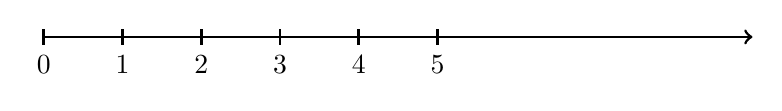
\begin{tikzpicture}[line width=1pt]
		\draw [->] (0,0) --(9,0);
		\foreach \x in {0,1,...,5}
		\draw (\x,0.1)--(\x,-0.1) node [below] {\x};
	\end{tikzpicture}
	\vspace*{-10pt}
\end{figure}
-- Trong hai số tự nhiên khác nhau, luôn có một số nhỏ hơn số kia. Trên tia số, số nào gần số 0 hơn thì số đó bé hơn.

-- Mỗi số tự nhiên khác 0 đều có một số liền trước và một số liền sau.

-- Mỗi số tự nhiên viết trong hệ thập phân đều biểu diễn được thành tổng các giá trị chữ số của nó. Ví dụ $234=2\times 100+3\times 10+4$

\subsection{THỰC HÀNH GIẢI TOÁN}
\begin{vd}
	Cho tập hợp $P=\left\{ x\in N\left| 4\le x<\left. 12 \right\} \right. \right.$ và tập hợp Q là những số tự nhiên chẵn có một chữ số.
	
	$a)$ Trong những số 0; 2; 6; 9; 12 số nào thuộc tập hợp $P$, số nào không thuộc tập hợp $P$? Dùng kí hiệu để trả lời.
	
	$b)$ Viết tập hợp $Q$ bằng cách liệt kê phần tử.
	
	$c)$ Chỉ ra những phần tử thuộc cả hai tập hợp $P$ và $Q$.
	
	$d)$ Gọi $M$ là tập hợp các số lẻ thuộc tập $P$. Hãy viết tập hợp $M$ bằng $2$ cách.
	\loigiai{
	\textbf{\textit{Tìm cách giải}}
	
	$a)$ Nêu tính chất đặc trưng của các phần tử thuộc tập $P$. Trong các số đã cho, số nào có tính chất ấy? Số nào không có tính chất ấy?
	
	$b)$ Đọc các số tự nhiên chẵn có một chữ số theo thứ tự từ bé đến lớn. 
	
	$c)$ Viết tập hợp $P$ bằng cách liệt kê phần tử. Từ đó chỉ ra những phần tử thuộc cả hai tập hợp $P$ và $Q$.
	
	$d)$ Từ tập hợp $P$, hãy đọc các số lẻ thuộc tập hợp $P$.
	 
	\textbf{\textit{Trình bày lời giải}}
	
	$a)$ $0\notin P$, $2\notin P$, $6\in P$, $9\in P$, $12\notin P$.
	
	$b)$ $P=\{4;5;6;7;8;9;10;11\}$;
	
	$Q=\{0;2;4;6;8\}$.
	
	$c)$ Gọi $R$ là tập hợp gồm những phần tử thuộc cả hai tập hợp $P$ và $Q$. Ta có: $R=\{4;6;8\}$
	
	$d)$ Cách $1$: $M=\{ 5;7;9;11\}$.
	
	Cách $2$: $M=\left\{x \mid x \text{ là số tự nhiên lẻ và } 5\le x\le 11 \right\}$.
	}
\end{vd}

\begin{vd}
	Cho các số tự nhiên 5, 37, 149.
	
	$a)$ Hãy viết các số đó bằng số La Mã.
	
	$b)$ Hãy biểu diễn các số đó trong hệ thập phân.
	
	$c)$ Trong các số trên, số nào viết được dưới dạng $5\times a+4\times b$trong đó $a$ và $b$ là các số tự nhiên khác 0?
	\loigiai{
	$a)$ \begin{center}
		\renewcommand{\arraystretch}{1.25}
		\begin{tabular}{|l|c|c|c|}
			\hline
			Giá trị trong hệ thập phân&	5	&37&	149\\
			\hline
			Viết bằng số La Mã&	V&	XXXVII	&CXLIX\\
			\hline
		\end{tabular}
	\end{center}
	$b)$ 5 là số có một chữ số nên không cần biểu diễn:
	\begin{align*}
		37&=3\times 10+7\\
		149&=1\times 100+4\times 10+9
	\end{align*}
	$c)$ Vì $a$ và $b$ là các số tự nhiên khác $0$ nên $5\times a+4\times b>9$.
	
	Do đó, $5$ không viết được dưới dạng trên.
	
	Nhận thấy $37=5\times 5+4\times 3$; $149=29\times 5+4\times 1$.
	
	Vậy chỉ có $37$ và $149$ viết được dưới dạng $5\times a+4\times b$.
	
	\textit{Nhận xét. chỉ có 37 và 149 còn viết được dưới dạng $5\times a+4\times b$ bằng cách khác, các bạn hãy thử xem?}
	}
\end{vd}

\begin{vd}
	Một cuốn sách toán có $200$ trang. Hỏi phải cần bao nhiêu chữ số để đánh số trang của cuốn sách đó biết rằng cuốn sách đó được đánh số trang bắt đầu từ trang thứ 3?
	\loigiai{
	Từ trang 3 đến trang 9 dùng hết: $\left( 9-3 \right)+1=7$ (chữ số).
	
	Từ trang 10 đến trang 99 có: $\left( 99-10 \right)+1=90$ (trang). Số chữ số cần dùng là: $90\times 2=180$ (chữ số).
	
	Từ trang 100 đến trang 200 có: $\left( 200-100 \right)+1=101$ (trang). Số chữ số cần dùng là $101\times 3=303$ (chữ số).
	
	Vậy để đánh số trang cho cuốn sách trên cần:
	\[7+180+303=490 \text{ (chữ số).}\]
	Từ số tự nhiên $a$ đến số tự nhiên $b$ ($a<b$) có: $b-a+1$ số tự nhiên (tính cả $a$ và $b$).
	}
\end{vd}

\subsection{MỞ RỘNG KIẾN THỨC}
-- Tập hợp không có phần tử nào gọi là tập rỗng. Ví dụ: Tập hợp $A$ gồm các số tự nhiên nhỏ hơn $0$. Tập rỗng kí hiệu là: $\varnothing $

-- Nếu mọi phần tử của tập hợp $A$ đều có trong tập hợp $B$ thì ta nói tập hợp $A$ là con của tập hợp $B$. Kí hiệu $A\subset B$ hoặc $B\supset A$ (đọc là $B$ chứa $A$).
\begin{center}
	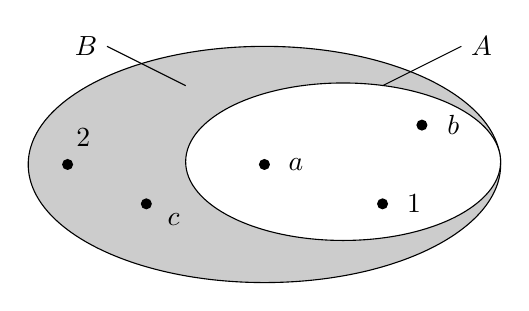
\begin{tikzpicture}[scale=1]
		\draw[fill=gray!40]
		(0:0) ellipse ({3} and {1.5})
		;
		\draw[fill=white]
		(2:1) ellipse ({2} and {1})
		;
		\draw
		(-2,1.5) node[left]{$B$}--(-1,1)
		(2.5,1.5) node[right]{$A$}--(1.5,1)
		;
		\path
		(0,0) coordinate (a)
		(1.5,-.5) coordinate (1)
		(2,.5) coordinate (b)
		(-2.5,0) coordinate (2)
		(-1.5,-.5) coordinate (c)
		;
		\foreach \i/\g in {a/0,b/0,1/0,2/60, c/-30}\fill[black] (\i) circle (2pt) +(\g:.4) node{$\i$};
	\end{tikzpicture}
\end{center}
\textit{Dựa vào hình vẽ ta thấy, tập hợp $A$ gồm $3$ phần tử là $a$; $b$; 1 đều thuộc tập hợp $B$. Ta nói tập hợp $A$ là con của tập hợp $B$.}
\begin{ly}
	\begin{itemize}
		\item	Mọi tập hợp đểu là tập hợp con của chính nó.
		
		\item	Quy ước $\varnothing \subset A$ với mọi $A$.
		
		\item	Nếu $A\subset B$ và $B\subset A$ thì $A = B$.
	\end{itemize}
\end{ly}


\subsection{BÀI TẬP TỰ LUYỆN}
\Opensolutionfile{loigiaichung}[loigiaichuong1]
\subsubsection*{Mức độ cơ bản}
\begin{bt}
	Cho tập hợp $A$ gồm những con vật có bốn chân
	
	$a)$ Trong các con vật Chó; Gà; Lợn; Chim Bồ Câu; Rắn, con vật nào thuộc tập hợp $A$, con vật nào không thuộc tập hợp $A$? Dùng kí hiệu để trả lời.
	
	$b)$ Hãy kể tên thêm $3$ phần tử thuộc tập hợp $A$?
	\begin{loigiaichuong1}
			$a)$ Các con vật có $4$ chân là Chó và Lợn.
			
			Do đó: Chó $\in A$; Gà $\notin A$; Lợn$ \in A$; Chim bồ câu $\notin A$; Rắn $\notin A$.
			
			$b)$ 3 phần tử thuộc tập hợp $A$ là: Trâu; Bò; Ngựa.
	\end{loigiaichuong1}
\end{bt}

\begin{bt}
	Viết các tập hợp sau bằng cách liệt kê phần tử
	
	$a)$ Tập hợp $T$ gồm các chữ cái trong từ SÁCH TOÁN 6.
	
	$b)$ Tập hợp $V$ gồm các tháng có 31 ngày trong một năm.
	\loigiai{
	$a)$	$T = \{S; A; C; H; T; O; N \}$.
	
	$b)$	$V =\{\text{tháng 1; tháng 3; tháng 5; tháng 7; tháng 8; tháng 10; tháng 12}\}$.
	}
\end{bt}
\begin{bt}
	Gọi $M$ là tập hợp gồm các số tự nhiên $y$ sao cho $y+1<6$. Hãy viết tập hợp M bằng hai cách.
	\begin{loigiaichuong1}
		$\bullet$	Cách 1: $M = \{0; 1; 2; 3; 4\}$.
		
		$\bullet$	Cách 2: $M = \{ y \mid y \in \mathbb{N},\, m y + 1 < 6\}$.
	\end{loigiaichuong1}
\end{bt}
\begin{bt}
	Điền vào chỗ trống
	\begin{center}
		\renewcommand{\arraystretch}{1.1}
		\begin{tabularx}{\textwidth}{|p{2cm}|*{6}{Y|} }
			\hline
			Số tự nhiên&	19&	&	&	74&	&	187\\
			\hline
			Số la mã&	&	XXIX&	LXII&	&	CLIV&	\\
			\hline
		\end{tabularx}
	\end{center}
	\begin{loigiaichuong1}
		\,\\
			\renewcommand{\arraystretch}{1.1}
			\begin{tabularx}{\textwidth}{|p{2cm}|*{6}{Y|} }
				\hline
				Số tự nhiên&	19&	\textbf{29} & \textbf{62}	&	74&	\textbf{154}&	187\\
				\hline
				Số la mã&	\textbf{XIX}&	XXIX&	LXII&	\textbf{LXXIV}&	CLIV&	\textbf{CLXXXVII}\\
				\hline
			\end{tabularx}
	\end{loigiaichuong1}	
\end{bt}
\begin{bt}
	Tìm các số liền trước và liền sau của 14, 898, 999
	\begin{loigiaichuong1}
		$\bullet$	Số liền trước của các số 14, 898, 999 lần lượt là: 13, 897, 998.
		
		$\bullet$	Số liền sau của các số 14, 898, 999 lần lượt là: 15, 899, 1000.
	\end{loigiaichuong1}
\end{bt} 
\begin{bt}
	Hãy chỉ ra tính chất đặc trưng cho các phần tử của các tập hợp sau đây
	
	$a)$ $A = \{0; 3; 6; 9; \ldots; 99\}$
	
	$b)$ $B = \{100; 200; 300; \ldots; 900\}$
	
	$c)$ $C = \{1; 5; 9; 13; 17;\ldots; 49\}$
	\begin{loigiaichuong1}
		$a)$	Tính chất đặc trưng của các phần tử thuộc tập hợp $A$ là: là số tự nhiên, chia hết cho 3 và nhỏ hơn 100.
		
		$b)$	Tính chất đặc trưng của các phần tử thuộc tập hợp $B$ là: là số tự nhiên tròn trăm và nhỏ hơn 1000.
		
		$c)$	Tính chất đặc trưng của các phần tử thuộc tập hợp $C$ là: là số tự nhiên liền sau của các số tự nhiên chia hết cho 4 và nhỏ hơn 50.
	\end{loigiaichuong1}
\end{bt}
\begin{bt}
	Biểu diễn các tập hợp sau bằng cách liệt kê các phần tử
	
	$a)$ $S=\left\{x \mid x \in \mathbb{N},\,2<x<9 \right\}$
	
	$b)$ $P=\left\{ y \mid y \in \mathbb{N^*},\, x\le 7 \right\}$
	
	$c)$ Tập hợp $Q$ gồm những phần tử thuộc cả $S$ và $P$ ở các ý trên.
	\begin{loigiaichuong1}
		Các tập hợp được viết dưới dạng liệt kê là:
		
		$a)$ $S = \{3; 4; 5; 6; 7; 8\}$.
		
		$b)$ $P = \{1; 2; 3; 4; 5; 6; 7\}$.
		
		$c)$ $Q = \{3; 4; 5; 6; 7\}$.
	\end{loigiaichuong1}
\end{bt}
\begin{bt}
	Hình vẽ dưới đây là hình vuông kích thước $4\times 4$ được chia thành 4 hình vuông nhỏ kích thước $2\times 2$. Trong các số tự nhiên từ 1 đến 4, em hãy chọn số thích hợp điền vào các ô vuông còn lại (không cần đúng thứ tự) sao cho: hàng dọc không có hai số nào trùng nhau, hàng ngang không có số nào trùng nhau và trong hình vuông $2\times 2$ cũng không có số nào trùng nhau (Trò chơi Sodoku).
	\begin{center}
		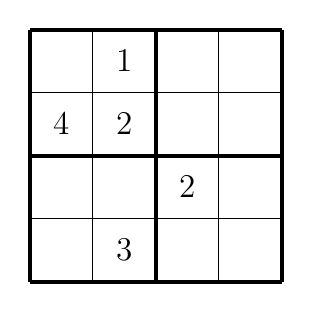
\begin{tikzpicture}[scale=0.8]
			\foreach \x in {0,2,4} \draw[line width=1.5pt] (\x,0)--(\x,-4);
			\foreach \x in {0,-2,-4} \draw[line width=1.5pt] (0,\x)--(4,\x);
			\foreach \x in {1,3} \draw (\x,0)--(\x,-4);
			\foreach \x in {-1,-3} \draw (0,\x)--(4,\x);
			\draw
			(1.5, -.5) node{\large $1$}
			(.5, -1.5) node{\large $4$}
			(1.5, -1.5) node{\large $2$}
			(1.5, -3.5) node{\large $3$}
			(2.5, -2.5) node{\large $2$};
		\end{tikzpicture}
	\end{center}
	\begin{loigiaichuong1}
	\,\\
	\begin{center}
		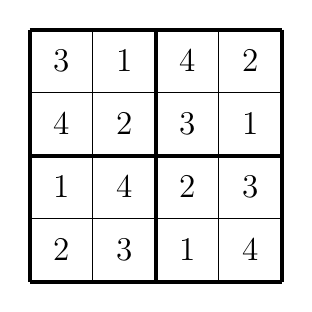
\begin{tikzpicture}[scale=0.8]
		\foreach \x in {0,2,4} \draw[line width=1.5pt] (\x,0)--(\x,-4);
		\foreach \x in {0,-2,-4} \draw[line width=1.5pt] (0,\x)--(4,\x);
		\foreach \x in {1,3} \draw (\x,0)--(\x,-4);
		\foreach \x in {-1,-3} \draw (0,\x)--(4,\x);
		\draw
		(1.5, -.5) node{\large $1$}
		(.5, -1.5) node{\large $4$}
		(1.5, -1.5) node{\large $2$}
		(1.5, -3.5) node{\large $3$}
		(2.5, -2.5) node{\large $2$}
		(.5, -.5) node{\large \bf $3$}
		(1.5, -2.5) node{\large \bf $4$}
		(.5, -2.5) node{\large \bf $1$}
		(.5, -3.5) node{\large \bf $2$}
		(3.5, -2.5) node{\large \bf $3$}
		(2.5, -1.5) node{\large $3$}
		(3.5, -1.5) node{\large \bf $1$}
		(2.5, -.5) node{\large \bf $4$}
		(3.5, -.5) node{\large \bf $2$}
		(2.5, -3.5) node{\large \bf $1$}
		(3.5, -3.5) node{\large \bf $4$}
		;
	\end{tikzpicture}
	\end{center}	
	\end{loigiaichuong1}
\end{bt}
\subsubsection*{Mức độ nâng cao}
\vspace*{-10pt}
\begin{bt}
	Cho tập hợp $P=\left\{ 3,5,7 \right\}$. 
	
	$a)$ Hãy tìm tất cả các tập hợp con của $P$ có: 1 phần tử, 2 phần tử, 3 phần tử
	
	$b)$ Tập hợp $P$ có tất cả bao nhiêu tập hợp con?
	\begin{loigiaichuong1}
		$a)$	Các tập hợp con của $P$ có
		
		$\bullet$	1 phần tử là: $\{3\}$; $\{5\}$; $\{7\}$.
		
		$\bullet$	2 phần tử là: $\{3; 5\}$; $\{3; 7\}$; $\{5; 7\}$.
		
		$\bullet$	3 phần tử là: $\{3; 5; 7\}$.
		
		$b)$	Tập hợp rỗng cũng là tập con của tập hợp $P$. Do đó, tập hợp $P$ có tất cả 8
		tập hợp con.
	\end{loigiaichuong1}
\end{bt}
\begin{bt}
	Để đánh số trang của một cuốn sách toán, người ta đã dùng hết 593 chữ số. Biết rằng cuốn sách đó được đánh số trang bắt đầu từ trang thứ 3. Hỏi cuốn sách đó có bao nhiêu trang?
	\begin{loigiaichuong1}
		Từ trang 3 đến trang 9 dùng hết:
		\[(9 - 3) + 1 = 7 \text{(chữ số)}.\]
		Từ 10 đến 99 có: $(99 - 10) + 1 = 90$ (số). Do đó, số chữ số cần dùng là:
		\[90 \times 2 = 180 \text{(chữ số)}.\]
		Khi đó còn lại: $592 - 7 - 180 = 405 < 900$ (chữ số). Do đó số trang của cuốn sách là một số có 3 chữ số.
		
		Số trang sách kể từ 100 trở đi của cuốn sách đó là:
		\[405 : 3 = 135 \text{(trang)}.\]
		Khi đó, số trang của cuốn sách là
		\[100 + 135 - 1 = 234 \text{(trang)}.\]
		Vậy cuốn sách đó có 234 trang.
	\end{loigiaichuong1}
\end{bt}
\begin{bt}
	Đội tuyển đấu cờ của Trường THCS Đa Tốn có 24 em, trong đó có 15 em thi đấu cờ vua và 11 em thi đấu cờ tướng. Hỏi có bao nhiêu em trong đội tuyển thi đấu cả hai môn?
	\begin{loigiaichuong1}
		Vì có 15 em thi đấu cờ vua trong 24 em của đội tuyển đấu cờ nên số em chỉ thi đấu cờ tướng là:
		\[24 - 15 = 9 \text{(em)}.\]
		Vì có 11 em thi đấu cờ tướng trong 24 em của đội tuyển đấu cờ nên số em chỉ thi đấu cờ vua là:
		\[24 - 11 = 13 \text{(em)}.\]
		Do đó, số em trong đội tuyển thi đấu cả hai môn là:
		\[11 - 9 = 2 = 15 - 13 \text{(em)}.\]
		Vậy có 2 em trong đội tuyển thi đấu cả hai môn.
	\end{loigiaichuong1}
\end{bt}
\begin{bt}
	Trong một hội nghị có 100 đại biểu tham dự. Mỗi đại biểu nói được một hoặc hai hoặc ba thứ tiếng: Đức, Anh hoặc Pháp. Biết rằng có 39 đại biểu chỉ nói được tiếng Anh, 35 đại biểu nói được tiếng Pháp, 8 đại biểu nói được cả tiếng Anh và tiếng Đức. Hỏi có bao nhiêu đại biểu chỉ nói được tiếng Đức?
	\begin{loigiaichuong1}
		Gọi $A$ là tập hợp các đại biểu nói được tiếng Anh, $Đ$ là tập hợp các đại biểu nói được tiếng Đức, $P$ là tập hợp các đại biểu nói được tiếng Pháp. Ta có sơ đồ:
		\begin{center}
			\begin{tikzpicture}[scale=0.8]
				\draw
				(0:0) ellipse ({2.5} and {1.5})
				;
				\draw
				(-1,-2) circle (2cm);
				\draw
				(4:-2) ellipse ({2.5} and {1.5})
				;
				\draw
				(-4,1.5) node[left]{A}--(-3,1)
				(2.5,1.5) node[right]{Đ}--(1.5,1)
				(1.2,-3) node[right]{P}--(0,-2.5)
				;
				%	\foreach \i/\g in {a/0,b/0,1/0,2/60, c/-30}\fill[black] (\i) circle (2pt) +(\g:.4) node{$\i$};
			\end{tikzpicture}
		\end{center}
		Vì $39$ đại biểu nói được tiếng Pháp nên số đại biểu không nói được tiếng Pháp là
		\[100 - 39 = 61 \text{(đại biểu)}.\]
		Các đại biểu không nói được tiếng Pháp bao gồm: các đại biểu chỉ nói được tiếng Anh, các đại biểu chỉ nói được tiếng Đức, các đại biểu nói được cả hai tiếng Anh và Đức (không nói được tiếng Pháp).
		
		Vì 35 đại biểu chỉ nói được tiếng Anh và 8 đại biểu nói được cả hai tiếng Anh và Đức (không nói được tiếng Pháp) nên số đại biểu chỉ nói được tiếng Đức là:
		\[61 - 35 - 8 = 18 \text{(đại biểu)}.\]
		Vậy có 18 đại biểu chỉ nói được tiếng Đức.	 
	\end{loigiaichuong1}
\end{bt}
\begin{bt}
	Hoàn thành trò chơi Sodoku sau
	\begin{center}
		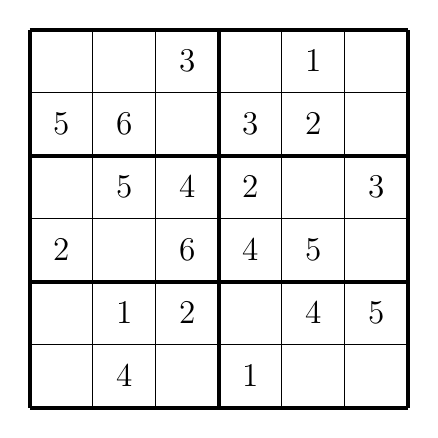
\begin{tikzpicture}[scale=0.8]
			\foreach \x in {0,3,6} \draw[line width=1.5pt] (\x,0)--(\x,6);
			\foreach \x in {0,2,4,6} \draw[line width=1.5pt] (0,\x)--(6,\x);
			\foreach \x in {1,2,4,5} \draw (\x,0)--(\x,6);
			\foreach \x in {1,3,5} \draw (0,\x)--(6,\x);
			\draw
			(1.5, .5) node{\large $4$}
			(3.5, .5) node{\large $1$}
			%
			(1.5, 1.5) node{\large $1$}
			(2.5, 1.5) node{\large $2$}
			(4.5, 1.5) node{\large $4$}
			(5.5, 1.5) node{\large \bf $5$}
			%
			(0.5, 2.5) node{\large \bf $2$}
			(2.5, 2.5) node{\large \bf $6$}
			(3.5, 2.5) node{\large \bf $4$}
			(4.5, 2.5) node{\large \bf $5$}
			%
			(1.5, 3.5) node{\large $5$}
			(2.5, 3.5) node{\large \bf $4$}
			(3.5, 3.5) node{\large \bf $2$}
			(5.5, 3.5) node{\large \bf $3$}
			%
			(.5, 4.5) node{\large \bf $5$}
			(1.5, 4.5) node{\large \bf $6$}
			(3.5, 4.5) node{\large \bf $3$}
			(4.5, 4.5) node{\large \bf $2$}
			%
			(2.5, 5.5) node{\large \bf $3$}
			(4.5,5.5) node{\large \bf $1$}
			;
		\end{tikzpicture}
		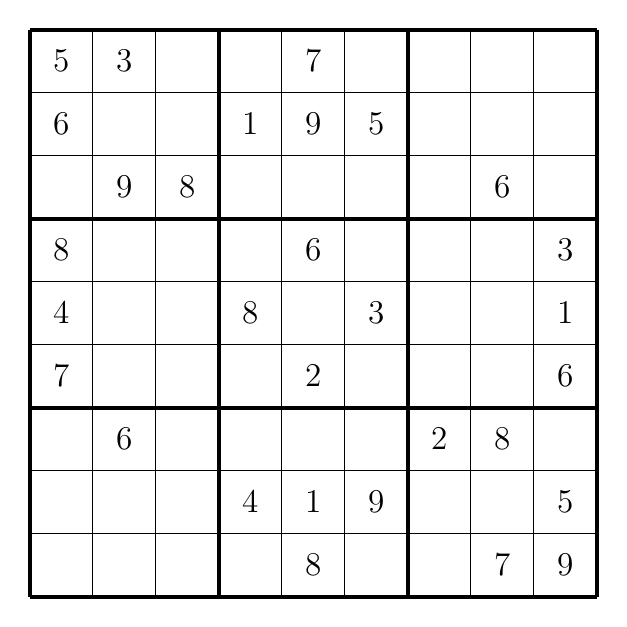
\begin{tikzpicture}[scale=.8]
			\foreach \x in {0,3,6,9} \draw[line width=1.5pt] (\x,0)--(\x,9);
			\foreach \x in {0,3,6,9} \draw[line width=1.5pt] (0,\x)--(9,\x);
			\foreach \x in {1,2,4,5,7,8} \draw (\x,0)--(\x,9);
			\foreach \x in {1,2,4,5,7,8} \draw (0,\x)--(9,\x);
			\draw
			(4.5, .5) node{\large $8$}
			(7.5, .5) node{\large $7$}
			(8.5, .5) node{\large $9$}
			%
			(3.5, 1.5) node{\large $4$}
			(4.5, 1.5) node{\large $1$}
			(5.5, 1.5) node{\large $9$}
			(8.5, 1.5) node{\large \bf $5$}
			%
			(1.5, 2.5) node{\large \bf $6$}
			(6.5, 2.5) node{\large \bf $2$}
			(7.5, 2.5) node{\large \bf $8$}
			%
			(0.5, 3.5) node{\large $7$}
			(4.5, 3.5) node{\large \bf $2$}
			(8.5, 3.5) node{\large \bf $6$}
			%
			(0.5, 4.5) node{\large \bf $4$}
			(3.5, 4.5) node{\large \bf $8$}
			(5.5, 4.5) node{\large \bf $3$}
			(8.5, 4.5) node{\large \bf $1$}
			%
			(0.5, 5.5) node{\large \bf $8$}
			(4.5,5.5) node{\large \bf $6$}
			(8.5,5.5) node{\large \bf $3$}
			%
			(1.5,6.5) node{\large \bf $9$}
			(2.5,6.5) node{\large \bf $8$}
			(7.5,6.5) node{\large \bf $6$}
			%
			(0.5,7.5) node{\large \bf $6$}
			(3.5,7.5) node{\large \bf $1$}
			(4.5,7.5) node{\large \bf $9$}
			(5.5,7.5) node{\large \bf $5$}
			%
			(0.5,8.5) node{\large \bf $5$}
			(1.5,8.5) node{\large \bf $3$}
			(4.5,8.5) node{\large \bf $7$}
			;
		\end{tikzpicture}
	\end{center}
	\begin{loigiaichuong1}
		\,\\
		\begin{center}
			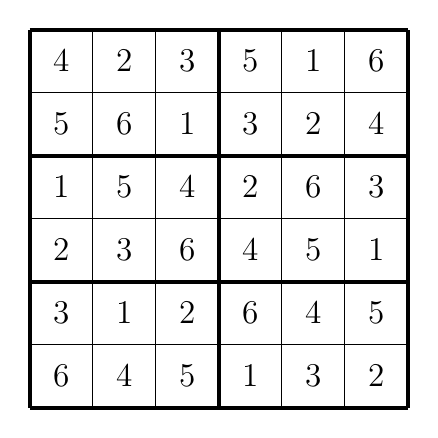
\begin{tikzpicture}[scale=0.8]
			\foreach \x in {0,3,6} \draw[line width=1.5pt] (\x,0)--(\x,6);
			\foreach \x in {0,2,4,6} \draw[line width=1.5pt] (0,\x)--(6,\x);
			\foreach \x in {1,2,4,5} \draw (\x,0)--(\x,6);
			\foreach \x in {1,3,5} \draw (0,\x)--(6,\x);
			\draw
			(1.5, .5) node{\large $4$}
			(3.5, .5) node{\large $1$}
			%
			(1.5, 1.5) node{\large $1$}
			(2.5, 1.5) node{\large $2$}
			(4.5, 1.5) node{\large $4$}
			(5.5, 1.5) node{\large \bf $5$}
			%
			(0.5, 2.5) node{\large \bf $2$}
			(2.5, 2.5) node{\large \bf $6$}
			(3.5, 2.5) node{\large \bf $4$}
			(4.5, 2.5) node{\large \bf $5$}
			%
			(1.5, 3.5) node{\large $5$}
			(2.5, 3.5) node{\large \bf $4$}
			(3.5, 3.5) node{\large \bf $2$}
			(5.5, 3.5) node{\large \bf $3$}
			%
			(.5, 4.5) node{\large \bf $5$}
			(1.5, 4.5) node{\large \bf $6$}
			(3.5, 4.5) node{\large \bf $3$}
			(4.5, 4.5) node{\large \bf $2$}
			%
			(2.5, 5.5) node{\large \bf $3$}
			(4.5,5.5) node{\large \bf $1$}
			%-----
			(0.5, 0.5) node{\large $6$}
			(2.5, 0.5) node{\large $5$}
			(4.5, 0.5) node{\large $3$}
			(5.5, 0.5) node{\large $2$}
			%
			(0.5, 1.5) node{\large $3$}
			(3.5, 1.5) node{\large $6$}
			%
			(1.5, 2.5) node{\large $3$}
			(5.5, 2.5) node{\large $1$}
			%
			(0.5, 3.5) node{\large $1$}
			(4.5, 3.5) node{\large $6$}
			%
			(2.5, 4.5) node{\large $1$}
			(5.5, 4.5) node{\large $4$}
			%
			(0.5, 5.5) node{\large $4$}
			(1.5, 5.5) node{\large $2$}
			(3.5, 5.5) node{\large $5$}
			(5.5, 5.5) node{\large $6$}
			;
		\end{tikzpicture}
		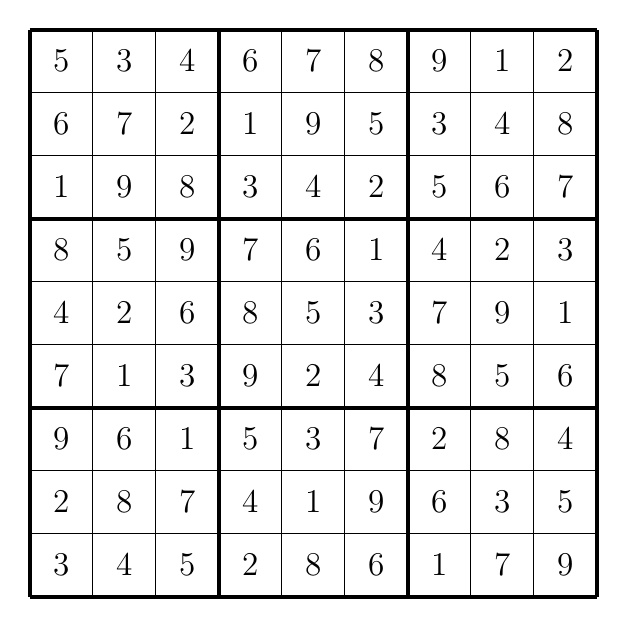
\begin{tikzpicture}[scale=.8]
			\foreach \x in {0,3,6,9} \draw[line width=1.5pt] (\x,0)--(\x,9);
			\foreach \x in {0,3,6,9} \draw[line width=1.5pt] (0,\x)--(9,\x);
			\foreach \x in {1,2,4,5,7,8} \draw (\x,0)--(\x,9);
			\foreach \x in {1,2,4,5,7,8} \draw (0,\x)--(9,\x);
			\draw
			(4.5, .5) node{\large $8$}
			(7.5, .5) node{\large $7$}
			(8.5, .5) node{\large $9$}
			%---
			(0.5, .5) node{\large $3$}
			(1.5, .5) node{\large $4$}
			(2.5, .5) node{\large $5$}
			(3.5, .5) node{\large $2$}
			(5.5, .5) node{\large $6$}
			(6.5, .5) node{\large $1$}
			%
			(3.5, 1.5) node{\large $4$}
			(4.5, 1.5) node{\large $1$}
			(5.5, 1.5) node{\large $9$}
			(8.5, 1.5) node{\large \bf $5$}
			%---
			(0.5, 1.5) node{\large $2$}
			(1.5, 1.5) node{\large $8$}
			(2.5, 1.5) node{\large $7$}
			(6.5, 1.5) node{\large \bf $6$}
			(7.5, 1.5) node{\large \bf $3$}
			%
			(1.5, 2.5) node{\large \bf $6$}
			(6.5, 2.5) node{\large \bf $2$}
			(7.5, 2.5) node{\large \bf $8$}
			%---
			(0.5, 2.5) node{\large \bf $9$}
			(2.5, 2.5) node{\large \bf $1$}
			(3.5, 2.5) node{\large \bf $5$}
			(4.5, 2.5) node{\large \bf $3$}
			(5.5, 2.5) node{\large \bf $7$}
			(8.5, 2.5) node{\large \bf $4$}
			%
			(0.5, 3.5) node{\large $7$}
			(4.5, 3.5) node{\large \bf $2$}
			(8.5, 3.5) node{\large \bf $6$}
			%---
			(1.5, 3.5) node{\large $1$}
			(2.5, 3.5) node{\large \bf $3$}
			(3.5, 3.5) node{\large \bf $9$}
			(5.5, 3.5) node{\large $4$}
			(6.5, 3.5) node{\large \bf $8$}
			(7.5, 3.5) node{\large \bf $5$}
			%
			(0.5, 4.5) node{\large \bf $4$}
			(3.5, 4.5) node{\large \bf $8$}
			(5.5, 4.5) node{\large \bf $3$}
			(8.5, 4.5) node{\large \bf $1$}
			%---
			(1.5, 4.5) node{\large \bf $2$}
			(2.5, 4.5) node{\large \bf $6$}
			(4.5, 4.5) node{\large \bf $5$}
			(6.5, 4.5) node{\large \bf $7$}
			(7.5, 4.5) node{\large \bf $9$}
			%
			(0.5, 5.5) node{\large \bf $8$}
			(4.5,5.5) node{\large \bf $6$}
			(8.5,5.5) node{\large \bf $3$}
			%---
			(1.5, 5.5) node{\large \bf $5$}
			(2.5,5.5) node{\large \bf $9$}
			(3.5,5.5) node{\large \bf $7$}
			(5.5, 5.5) node{\large \bf $1$}
			(6.5,5.5) node{\large \bf $4$}
			(7.5,5.5) node{\large \bf $2$}
			%
			(1.5,6.5) node{\large \bf $9$}
			(2.5,6.5) node{\large \bf $8$}
			(7.5,6.5) node{\large \bf $6$}
			%---
			(0.5,6.5) node{\large \bf $1$}
			(3.5,6.5) node{\large \bf $3$}
			(4.5,6.5) node{\large \bf $4$}
			(5.5,6.5) node{\large \bf $2$}
			(6.5,6.5) node{\large \bf $5$}
			(8.5,6.5) node{\large \bf $7$}
			%
			(0.5,7.5) node{\large \bf $6$}
			(3.5,7.5) node{\large \bf $1$}
			(4.5,7.5) node{\large \bf $9$}
			(5.5,7.5) node{\large \bf $5$}
			%---
			(1.5,7.5) node{\large \bf $7$}
			(2.5,7.5) node{\large \bf $2$}
			(6.5,7.5) node{\large \bf $3$}
			(7.5,7.5) node{\large \bf $4$}
			(8.5,7.5) node{\large \bf $8$}
			%
			(0.5,8.5) node{\large \bf $5$}
			(1.5,8.5) node{\large \bf $3$}
			(4.5,8.5) node{\large \bf $7$}
			%---
			(2.5,8.5) node{\large \bf $4$}
			(3.5,8.5) node{\large \bf $6$}
			(5.5,8.5) node{\large \bf $8$}
			(6.5,8.5) node{\large \bf $9$}
			(7.5,8.5) node{\large \bf $1$}
			(8.5,8.5) node{\large \bf $2$}
			;
		\end{tikzpicture}
		\end{center}
	\end{loigiaichuong1}
\end{bt}
\begin{bt}
	Có bao nhiêu số lẻ có 3 chữ số $\overline{abc}$ thỏa mãn $a<b\le c$ và $a+b+c=21$?
	\begin{loigiaichuong1}
		Vì $abc$ là số lẻ nên $c \in \{1; 3; 5; 7; 9\}$.
		
		Do $a < b \le c$ và $a + b + c = 21$ nên ta xét $c = 9$ trước. Khi đó, ta có các trường hợp:
		
		$\bullet$	$b = c = 9 \Rightarrow a = 3$. Ta được số 399.
		
		$\bullet$	$c = 9; b = 8 \Rightarrow a = 4$. Ta được số 489.
		
		$\bullet$	$c = 9; b = 7 \Rightarrow a = 5$. Ta được số 579.
		
		Xét $c = 7 \Rightarrow a = b = c = 7$ không thỏa mãn đề bài.
		
		Vậy có 3 số tự nhiên lẻ có ba chữ số thỏa mãn đề bài.
	\end{loigiaichuong1}
\end{bt}
\Closesolutionfile{loigiaichung}
